% Draft for an IEEE conference. Compile with pdfLaTeX + BibTeX (e.g. on Overleaf) or with tectonic.
% Numbers and result tables are generated: run  python scripts/make_paper_assets.py  after the notebooks.
\documentclass[conference]{IEEEtran}
\IEEEoverridecommandlockouts

\usepackage[T1]{fontenc}
\usepackage{cite}
\usepackage{amsmath,amssymb}
\usepackage{graphicx}
\usepackage{booktabs}
\usepackage{url}
\usepackage{xcolor}
\graphicspath{{../figures/}{figures/}}
\newcommand{\todo}[1]{\textcolor{red}{[TODO: #1]}}

% Generated by scripts/make_paper_assets.py from results/ - do not edit by hand.
\providecommand{\xspace}{}
\newcommand{\NRawPlayers}{50{,}149}
\newcommand{\NRawValuations}{656{,}301}
\newcommand{\NRawAppearances}{1{,}894{,}350}
\newcommand{\NRawTransfers}{175{,}165}
\newcommand{\NTransfersFee}{17{,}554}
\newcommand{\NValRowsLeakPeriod}{536{,}158}
\newcommand{\NValRowsNoTransfer}{207{,}325}
\newcommand{\PctValRowsNoTransfer}{38.7}
\newcommand{\PctNoTransferIsToday}{100}
\newcommand{\PctTransferIsTransfer}{100}
\newcommand{\PctContractFuture}{54.6}
\newcommand{\NCoreLeagues}{14}
\newcommand{\NNewLeagues}{17}
\newcommand{\CoreLeagueList}{BE1, DK1, ES1, FR1, GB1, GR1, IT1, L1, NL1, PO1, RU1, SC1, TR1, UKR1}
\newcommand{\NRows}{357{,}624}
\newcommand{\NPlayers}{35{,}897}
\newcommand{\NCoreRows}{136{,}653}
\newcommand{\NCorePlayers}{20{,}288}
\newcommand{\NTrain}{112{,}775}
\newcommand{\NVal}{11{,}711}
\newcommand{\NTest}{12{,}167}
\newcommand{\NTestPlayers}{6{,}292}
\newcommand{\NTune}{99{,}976}
\newcommand{\NNewLeagueRows}{8{,}671}
\newcommand{\NLeakChecks}{100}
\newcommand{\NLeakPassed}{100}
\newcommand{\NFeatures}{50}
\newcommand{\NUnknownRows}{76{,}130}
\newcommand{\NUnknownTest}{59}
\newcommand{\BaseRose}{35.4}
\newcommand{\BaseFell}{51.5}
\newcommand{\BaseSame}{13.0}
\newcommand{\MAENaive}{0.480}
\newcommand{\WithinNaive}{32.2}
\newcommand{\MdAPENaive}{37.5}
\newcommand{\MAERidge}{0.407}
\newcommand{\WithinRidge}{35.0}
\newcommand{\MdAPERidge}{30.5}
\newcommand{\SkillRidge}{15.1}
\newcommand{\RhoRidge}{0.56}
\newcommand{\PRiseRidge}{68.8}
\newcommand{\PFallRidge}{90.6}
\newcommand{\RsqChangeRidge}{0.32}
\newcommand{\VsCurveRidge}{3.6}
\newcommand{\MAERF}{0.400}
\newcommand{\WithinRF}{35.8}
\newcommand{\MdAPERF}{29.5}
\newcommand{\SkillRF}{16.6}
\newcommand{\RhoRF}{0.59}
\newcommand{\PRiseRF}{69.8}
\newcommand{\PFallRF}{96.5}
\newcommand{\RsqChangeRF}{0.36}
\newcommand{\VsCurveRF}{5.3}
\newcommand{\MAEXGB}{0.395}
\newcommand{\WithinXGB}{37.3}
\newcommand{\MdAPEXGB}{28.5}
\newcommand{\SkillXGB}{17.7}
\newcommand{\RhoXGB}{0.58}
\newcommand{\PRiseXGB}{71.7}
\newcommand{\PFallXGB}{95.2}
\newcommand{\RsqChangeXGB}{0.35}
\newcommand{\VsCurveXGB}{6.5}
\newcommand{\MAECat}{0.395}
\newcommand{\WithinCat}{37.6}
\newcommand{\MdAPECat}{28.1}
\newcommand{\SkillCat}{17.7}
\newcommand{\RhoCat}{0.58}
\newcommand{\PRiseCat}{72.1}
\newcommand{\PFallCat}{95.7}
\newcommand{\RsqChangeCat}{0.34}
\newcommand{\VsCurveCat}{6.6}
\newcommand{\MAELGB}{0.394}
\newcommand{\WithinLGB}{37.8}
\newcommand{\MdAPELGB}{28.1}
\newcommand{\SkillLGB}{17.9}
\newcommand{\RhoLGB}{0.58}
\newcommand{\PRiseLGB}{73.0}
\newcommand{\PFallLGB}{95.6}
\newcommand{\RsqChangeLGB}{0.33}
\newcommand{\VsCurveLGB}{6.8}
\newcommand{\MAEGRU}{0.397}
\newcommand{\WithinGRU}{37.8}
\newcommand{\MdAPEGRU}{28.2}
\newcommand{\SkillGRU}{17.2}
\newcommand{\RhoGRU}{0.57}
\newcommand{\PRiseGRU}{72.6}
\newcommand{\PFallGRU}{93.5}
\newcommand{\RsqChangeGRU}{0.33}
\newcommand{\VsCurveGRU}{6.0}
\newcommand{\MAEEns}{0.393}
\newcommand{\WithinEns}{38.0}
\newcommand{\MdAPEEns}{27.8}
\newcommand{\SkillEns}{18.1}
\newcommand{\RhoEns}{0.59}
\newcommand{\PRiseEns}{73.4}
\newcommand{\PFallEns}{95.0}
\newcommand{\RsqChangeEns}{0.34}
\newcommand{\VsCurveEns}{7.0}
\newcommand{\MAECurve}{0.423}
\newcommand{\WithinCurve}{35.3}
\newcommand{\MdAPECurve}{31.3}
\newcommand{\SkillCurve}{12.0}
\newcommand{\RhoCurve}{0.51}
\newcommand{\PRiseCurve}{63.6}
\newcommand{\PFallCurve}{92.6}
\newcommand{\RsqChangeCurve}{0.24}
\newcommand{\VsCurveLGBCI}{[6.0, 7.6]}
\newcommand{\VsCurveXGBCI}{[5.7, 7.4]}
\newcommand{\VsCurveCatCI}{[5.7, 7.4]}
\newcommand{\VsCurveRidgeCI}{[2.8, 4.3]}
\newcommand{\VsCurveRFCI}{[4.4, 6.2]}
\newcommand{\VsCurveGRUCI}{[5.1, 7.0]}
\newcommand{\SkillCurveCI}{[10.9, 13.0]}
\newcommand{\SkillLGBCI}{[16.8, 19.0]}
\newcommand{\SkillMomentum}{$-$33.3}
\newcommand{\SkillMomentumDamped}{$-$0.2}
\newcommand{\VsCurveLeagueCurve}{$-$0.2}
\newcommand{\VsCurveLeagueCurveCI}{[$-$0.7, 0.2]}
\newcommand{\MAEeurNaive}{2.89}
\newcommand{\MAEeurLGB}{2.45}
\newcommand{\RsqLevelNaive}{0.83}
\newcommand{\RsqLevelLGB}{0.89}
\newcommand{\GRUsd}{0.003}
\newcommand{\GRUepochs}{9}
\newcommand{\DiffLGBCurve}{$-$0.0286}
\newcommand{\DiffLGBCurveCI}{[$-$0.0322, $-$0.0250]}
\newcommand{\DiffLGBCat}{$-$0.0008}
\newcommand{\DiffLGBCatCI}{[$-$0.0018, 0.0002]}
\newcommand{\DiffLGBXGB}{$-$0.0010}
\newcommand{\DiffLGBXGBCI}{[$-$0.0022, 0.0002]}
\newcommand{\DiffCatXGB}{$-$0.0002}
\newcommand{\DiffCatXGBCI}{[$-$0.0015, 0.0012]}
\newcommand{\DiffLGBGRU}{$-$0.0033}
\newcommand{\DiffLGBGRUCI}{[$-$0.0053, $-$0.0013]}
\newcommand{\DiffLGBEns}{0.0009}
\newcommand{\DiffLGBEnsCI}{[$-$0.0001, 0.0020]}
\newcommand{\DiffLGBRF}{$-$0.0061}
\newcommand{\DiffLGBRFCI}{[$-$0.0087, $-$0.0035]}
\newcommand{\DiffLGBRidge}{$-$0.0135}
\newcommand{\DiffLGBRidgeCI}{[$-$0.0161, $-$0.0107]}
\newcommand{\SplitSkillTime}{17.1}
\newcommand{\SplitMAETime}{0.398}
\newcommand{\SplitSkillRows}{19.7}
\newcommand{\SplitMAERows}{0.359}
\newcommand{\SplitSkillPlayers}{17.5}
\newcommand{\SplitMAEPlayers}{0.373}
\newcommand{\SplitSkillRowsRecent}{23.8}
\newcommand{\SplitSkillPlayersRecent}{19.7}
\newcommand{\LeakLater}{82}
\newcommand{\LeakExact}{47}
\newcommand{\SplitDiffRowsTime}{2.6}
\newcommand{\SplitDiffRowsTimeCI}{[1.0, 4.3]}
\newcommand{\SplitDiffPlayersTime}{0.4}
\newcommand{\SplitDiffPlayersTimeCI}{[$-$1.2, 2.0]}
\newcommand{\SplitDiffRowsPlayers}{2.2}
\newcommand{\SplitDiffRowsPlayersCI}{[1.0, 3.4]}
\newcommand{\SplitDiffRowsTimeRecent}{6.7}
\newcommand{\SplitDiffRowsTimeRecentCI}{[3.8, 9.5]}
\newcommand{\SplitDiffPlayersTimeRecent}{2.6}
\newcommand{\SplitDiffPlayersTimeRecentCI}{[$-$0.6, 5.8]}
\newcommand{\SplitDiffRowsPlayersRecent}{4.1}
\newcommand{\SplitDiffRowsPlayersRecentCI}{[0.4, 7.8]}
\newcommand{\SkillAgeU}{17}
\newcommand{\SkillAgeA}{7}
\newcommand{\SkillAgeB}{15}
\newcommand{\SkillAgeC}{45}
\newcommand{\WithinAgeUNaive}{27.5}
\newcommand{\WithinAgeULGB}{21.8}
\newcommand{\SkillGK}{11}
\newcommand{\SkillCheap}{15}
\newcommand{\SkillExpensive}{20}
\newcommand{\MAEBigFallNaive}{0.66}
\newcommand{\MAEBigFallLGB}{0.44}
\newcommand{\MAEBigRiseNaive}{1.01}
\newcommand{\MAEBigRiseLGB}{0.78}
\newcommand{\MAEStableNaive}{0.02}
\newcommand{\MAEStableLGB}{0.19}
\newcommand{\SkillCoreLeagueMin}{8}
\newcommand{\SkillCoreLeagueMax}{29}
\newcommand{\SkillNewLeagueMin}{8}
\newcommand{\SkillNewLeagueMax}{24}
\newcommand{\NewLeagueNegative}{RSK1}
\newcommand{\SkillNewLeaguesLGB}{13.3}
\newcommand{\SkillOtherLGB}{12.2}
\newcommand{\UnknownModel}{CatBoost}
\newcommand{\MAEcoreWithoutUnknown}{0.3948}
\newcommand{\MAEcoreWithUnknown}{0.3948}
\newcommand{\ShapHist}{32}
\newcommand{\ShapClub}{27}
\newcommand{\ShapPlayer}{17}
\newcommand{\ShapPerf}{13}
\newcommand{\ShapTransfers}{10}
\newcommand{\ShapTopFive}{age, the change since the previous valuation, the value relative to the league median, the number of past valuations and the days since the last match}
\newcommand{\ShapFinRankMin}{33}
\newcommand{\ShapFinRankMax}{36}
\newcommand{\SpendTotalValueCorr}{0.91}
\newcommand{\SnapDiff}{0.0011}
\newcommand{\SnapDiffCI}{[0.00003, 0.0021]}
\newcommand{\AblHist}{0.0089}
\newcommand{\AblPerf}{0.0064}
\newcommand{\AblPlayer}{0.0052}
\newcommand{\AblClub}{0.0039}
\newcommand{\AblTransfers}{0.0004}
\newcommand{\AblFin}{0.0006}
\newcommand{\AblHistOnly}{0.0158}
\newcommand{\SkillHistOnly}{14.6}
\newcommand{\RollVsCurveMin}{3.6}
\newcommand{\RollVsCurveMax}{8.6}
\newcommand{\RollVsCurveMean}{5.8}
\newcommand{\RollVsCurveWins}{6}
\newcommand{\RollCurveMin}{6.6}
\newcommand{\RollCurveMax}{12.0}
\newcommand{\RollSkillMin}{11.5}
\newcommand{\RollSkillMax}{17.1}
\newcommand{\RollSkillMean}{14.5}
\newcommand{\RollRidgeMin}{9.7}
\newcommand{\RollRidgeMax}{15.1}
\newcommand{\RollYears}{6}
\newcommand{\RollLGBWins}{6}
\newcommand{\RollTrainFirst}{48{,}312}
\newcommand{\RollTrainLast}{112{,}775}
\newcommand{\UVRose}{73.0}
\newcommand{\UVRoseCI}{[70.2, 75.8]}
\newcommand{\YoungRose}{65.8}
\newcommand{\YoungRoseCI}{[62.8, 69.2]}
\newcommand{\AllRose}{35.4}
\newcommand{\OVFell}{95.6}
\newcommand{\UVSold}{16.4}
\newcommand{\AllSold}{17.3}
\newcommand{\UVFeeRatio}{2.5}
\newcommand{\AllFeeRatio}{0.88}
\newcommand{\YoungFeeRatio}{1.7}
\newcommand{\UVFeeAbove}{70}
\newcommand{\AllFeeAbove}{40}
\newcommand{\YoungFeeAbove}{69}
\newcommand{\UVAge}{20.3}
\newcommand{\GrpVsCurveU}{9.3}
\newcommand{\GrpVsCurveUCI}{[7.1, 11.5]}
\newcommand{\GrpVsCurveA}{6.6}
\newcommand{\GrpVsCurveACI}{[5.5, 7.7]}
\newcommand{\GrpVsCurveB}{6.3}
\newcommand{\GrpVsCurveBCI}{[4.7, 7.8]}
\newcommand{\GrpVsCurveC}{3.5}
\newcommand{\GrpVsCurveCCI}{[1.4, 5.8]}
\newcommand{\GrpVsCurveBigFall}{9.7}
\newcommand{\GrpVsCurveBigFallCI}{[8.4, 11.0]}
\newcommand{\GrpVsCurveModFall}{13.6}
\newcommand{\GrpVsCurveModFallCI}{[11.0, 16.1]}
\newcommand{\GrpVsCurveModRise}{$-$7.3}
\newcommand{\GrpVsCurveModRiseCI}{[$-$11.1, $-$3.8]}
\newcommand{\GrpVsCurveBigRise}{5.4}
\newcommand{\GrpVsCurveBigRiseCI}{[4.0, 6.6]}
\newcommand{\GrpVsCurveCheap}{5.4}
\newcommand{\GrpVsCurveCheapCI}{[4.0, 6.8]}
\newcommand{\GrpVsCurveExpensive}{6.9}
\newcommand{\GrpVsCurveExpensiveCI}{[4.8, 9.2]}
\newcommand{\GrpVsNaiveC}{45.1}
\newcommand{\GrpPosVsCurveMin}{5.8}
\newcommand{\GrpPosVsCurveMax}{7.3}
\newcommand{\CoreLgPosCount}{12}
\newcommand{\CoreLgNeg}{SC1}
\newcommand{\NewLgPosCount}{6}
\newcommand{\NewLgNegCount}{0}
\newcommand{\RankRiseLGB}{73.0}
\newcommand{\RankRiseYoung}{65.8}
\newcommand{\RankRiseDiff}{7.2}
\newcommand{\RankRiseDiffCI}{[4.2, 10.3]}
\newcommand{\RankFallLGB}{95.6}
\newcommand{\RankFallOld}{88.8}
\newcommand{\RankFallDiff}{6.7}
\newcommand{\RankFallDiffCI}{[4.4, 9.0]}
\newcommand{\RankRiseCurve}{63.6}
\newcommand{\FullWinRows}{7{,}409}
\newcommand{\FullWinVsNaive}{19.8}
\newcommand{\FullWinVsNaiveCI}{[18.6, 21.0]}
\newcommand{\FullWinVsCurve}{8.5}
\newcommand{\FullWinVsCurveCI}{[7.6, 9.6]}
\newcommand{\IntCovRaw}{77.6}
\newcommand{\IntCovRawCI}{[76.8, 78.5]}
\newcommand{\IntCovCal}{80.0}
\newcommand{\IntCovCalCI}{[79.2, 80.9]}
\newcommand{\IntWidthCal}{116}
\newcommand{\IntWidthIncrease}{7}
\newcommand{\IntPinballCal}{0.127}
\newcommand{\IntCovCalU}{77.6}
\newcommand{\IntCovCalUCI}{[75.2, 79.8]}
\newcommand{\IntCovCalC}{81.8}
\newcommand{\IntBelowC}{14.8}
\newcommand{\IntAboveC}{3.4}
\newcommand{\IntAboveU}{14.3}
\newcommand{\IntPinballRef}{0.137}
\newcommand{\IntPinballRaw}{0.127}
\newcommand{\NCalRows}{12{,}799}
\newcommand{\FeeRhoLGB}{0.40}
\newcommand{\FeeRhoLGBCI}{[0.35, 0.46]}
\newcommand{\FeeRhoCurve}{0.33}
\newcommand{\FeeRhoCurveCI}{[0.28, 0.39]}
\newcommand{\FeeRhoAge}{0.38}
\newcommand{\FeeRhoAgeCI}{[0.32, 0.43]}
\newcommand{\FeeRhoTrue}{0.57}
\newcommand{\FeeRhoTrueCI}{[0.53, 0.62]}
\newcommand{\FeeRhoDiffCurve}{0.07}
\newcommand{\FeeRhoDiffCurveCI}{[0.03, 0.11]}
\newcommand{\FeeRhoDiffAge}{0.03}
\newcommand{\FeeRhoDiffAgeCI}{[$-$0.01, 0.07]}
\newcommand{\FeeN}{2{,}100}
\newcommand{\FeePlayers}{1{,}121}
\newcommand{\DropRateTest}{25.5}
\newcommand{\DropTest}{2{,}530}
\newcommand{\DropTestComplete}{9{,}939}
\newcommand{\KeptPartial}{4{,}758}
\newcommand{\DropFell}{43}
\newcommand{\DropRose}{34}
\newcommand{\KeptFell}{41}
\newcommand{\KeptRose}{42}
\newcommand{\DropYoungMedian}{0.21}
\newcommand{\KeptYoungMedian}{0.41}
\newcommand{\NewWindowCov}{46.5}
\newcommand{\NewZeroMin}{87.3}
\newcommand{\CoreZeroMin}{4.7}
\newcommand{\NewNoApp}{72}
\newcommand{\NewVsCurve}{4.1}
\newcommand{\NewVsCurveCI}{[3.1, 5.1]}
\newcommand{\NewVsNaive}{13.3}
\newcommand{\NewNoPerfVsCurve}{2.1}
\newcommand{\NewNoPerfVsCurveCI}{[0.9, 3.2]}
\newcommand{\NewCurveVsNaive}{9.6}
\newcommand{\NResultTables}{55}
\newcommand{\NFigures}{15}
\newcommand{\PctTies}{5.3}

% Double-blind switch, read by main.tex and supplement.tex.
% \anonymoustrue  : submission version (no author block at all, no code link)
% \anonymousfalse : camera-ready version (real author block and GitHub link)
\newif\ifanonymous
\anonymoustrue
       % double-blind switch
\raggedbottom            % avoid stretched gaps between paragraphs

\begin{document}

\title{Forecasting Football Player Market Values One Year Ahead: A Leak-Checked Public Benchmark}

\ifanonymous
\author{}                % no author block in the submission version
\else
\author{\IEEEauthorblockN{Tasnim Nahar Raisa}
\IEEEauthorblockA{\textit{Department of Computer Science and Engineering} \\
\textit{International Islamic University Chittagong}\\
Chittagong, Bangladesh \\
tasnimraisa24@gmail.com}
}
\fi

\maketitle

\begin{abstract}
This paper sets up a free benchmark for predicting where a footballer's Transfermarkt market value will be 12 months later. Everything is built from a public Kaggle dataset and can be rerun from scratch. While preparing the data we found that some of its columns carry information from the future, so each of the \NFeatures{} features was tested to confirm it uses only data known on the valuation date. We split strictly by time. Under that split, an age $\times$ value lookup curve cuts the error of a no-change forecast by \SkillCurve\%. Gradient-boosted trees do better than the curve in all six test years we checked (\RollVsCurveMin{} to \RollVsCurveMax\% with fixed settings, and \VsCurveLGB\% \VsCurveLGBCI{} in 2024/25 after tuning). Most of their extra gain comes from players younger than 21 and from players whose value drops. If the data are split 80/20 at random instead, accuracy looks higher than it really is, largely because one player's records then sit in both training and test. After calibration, our 80\% forecast intervals contain the true value \IntCovCal\% of the time. On real transfer fees the forecasts beat the curve, but age by itself does about as well. A single script rebuilds all results from raw data with known checksums.
\end{abstract}

\begin{IEEEkeywords}
football analytics, market value, forecasting, benchmark, data leakage, time series evaluation, reproducibility
\end{IEEEkeywords}

% =============================================================================
\section{Introduction}

Transfermarkt publishes market values for tens of thousands of professional footballers. An online community sets these values. They are strongly related to actual transfer fees, although they are not unbiased predictors of them~\cite{coates2022wisdom}, and they have become the standard target for data-driven player valuation~\cite{mueller2017beyond,franceschi2024determinants}. What a club often needs, though, is a sense of where a value is heading. That question comes up when deciding whether to extend a contract or sell a player now.

Most machine learning studies estimate the current value or a transfer fee from attributes measured at the same time~\cite{mueller2017beyond,yigit2020xgboost,behravan2021novel,alasadi2022predict,aydemir2022ensembling,mchale2023estimating,huang2023explainable,tamim2025machine,fotache2026machine,wang2026predicting,li2026interpretable}. Only two recent studies forecast future values~\cite{baouan2025what,vanarem2025forecasting}, and one of them uses data that is not public. Results in this area are also hard to compare and easy to overstate, for three reasons. Random splits put the same player, and later time periods, in both training and test data. Public datasets store current attributes next to historical observations, which can leak future information~\cite{kapoor2023leakage}. And models are rarely compared with strong simple baselines or reported with confidence intervals.

This paper does not propose a new method. We build a 12-month forecasting benchmark from the free Kaggle Transfermarkt dataset~\cite{kaggle_transfermarkt} and audit the public data for leakage. Each feature was put through a cut-the-future test, and all results can be rebuilt from checksummed raw data with one script. For evaluation we hold out data by time, leave an embargo gap, compare against strong simple baselines, repeat the test over six rolling years and attach player-level bootstrap intervals to the numbers. We also put a figure on how far random splits inflate accuracy. The last part asks where machine learning actually beats an age $\times$ value curve. Here we look at calibrated forecast intervals, SHAP explanations and real transfer fees.

% =============================================================================
\section{Related Work}

Most machine learning work in team sports has gone into predicting match results~\cite{bunker2022application}. Player valuation has its own literature. Franceschi et al.~\cite{franceschi2024determinants} survey the factors that economists have linked to player value. Coates and Parshakov~\cite{coates2022wisdom} compared Transfermarkt's crowd estimates with real fees and found them useful, though biased. An early data-driven attempt came from M\"uller et al.~\cite{mueller2017beyond}, who fitted a multilevel regression to 4,217 players across six seasons of the five biggest European leagues.

Several later studies relied on video game and simulation data. Yigit et al.~\cite{yigit2020xgboost} combined XGBoost and lasso on Football Manager attributes of 5,316 players from 11 leagues. Behravan and Razavi~\cite{behravan2021novel} clustered FIFA~20 players by position and fitted a support vector regression, tuned with particle swarm optimisation, for each cluster. On FIFA~20 attributes, Al-Asadi and Ta\c{s}demir~\cite{alasadi2022predict} found that random forest worked best, and Huang and Zhang~\cite{huang2023explainable} used SHAP to explain tree ensembles trained on about 12,000 sofifa players.

Transfer fees have been modelled too. Aydemir et al.~\cite{aydemir2022ensembling} stacked LightGBM models on performance, popularity and transfer data. McHale and Holmes~\cite{mchale2023estimating} showed that advanced performance metrics and XGBoost improve fee predictions, and that the buying club's spending is a strong predictor. Poli et al.~\cite{poli2024statistical} used linear regression on more than 8,000 fees worldwide, while Li et al.~\cite{li2026interpretable} compared four models on about 800 Big-Five fees and explained them with SHAP.

Newer value models work with larger datasets. Tamim et al.~\cite{tamim2025machine} found random forest best on FIFA~22 attributes of more than 16,000 players, and Khalife et al.~\cite{khalife2025dynamic} fitted gradient boosting separately by age group and position. Fotache et al.~\cite{fotache2026machine} used about 14,000 player-seasons from FBref and Transfermarkt, where gradient boosting and neural networks performed best. Wang et al.~\cite{wang2026predicting} stacked gradient boosting models with an attention LSTM for 18,547 players of the top five leagues, and Zar\k{e}ba et al.~\cite{zareba2025decoding} valued defenders from event-based metrics with XGBoost and neural networks. A number of these studies evaluate with random splits or $k$-fold cross-validation~\cite{tamim2025machine,khalife2025dynamic,wang2026predicting}.

Two studies are closest to our question. Baouan et al.~\cite{baouan2025what} used lasso and random forests to select features that forecast future Transfermarkt values for each position. Van Arem et al.~\cite{vanarem2025forecasting} forecast how quality and value develop over time, with a time-based evaluation on non-public data.

\begin{table}[t]
\centering
\caption{Closest related studies. ``Current'' means the value or fee at the time of measurement. ``Future'' means the value at a later date.}
\label{tab:related}
\footnotesize
\setlength{\tabcolsep}{2.3pt}
\begin{tabular}{@{}llll@{}}
\toprule
Study & Data & Target & Main model \\
\midrule
\cite{mueller2017beyond} & Transfermarkt, top-5 leagues & current value & multilevel regression \\
\cite{yigit2020xgboost} & Football Manager (game) & current value & XGBoost + lasso \\
\cite{behravan2021novel} & FIFA 20 & current value & PSO-SVR \\
\cite{alasadi2022predict} & FIFA 20 (sofifa) & current value & random forest \\
\cite{aydemir2022ensembling} & performance, popularity & transfer fee & LightGBM stacking \\
\cite{mchale2023estimating} & advanced metrics & transfer fee & XGBoost \\
\cite{huang2023explainable} & sofifa, $\sim$12k players & current value & GBDT + SHAP \\
\cite{tamim2025machine} & FIFA 22, $>$16k players & current value & random forest \\
\cite{li2026interpretable} & $\sim$800 Big-Five fees & transfer fee & 4 models + SHAP \\
\cite{fotache2026machine} & FBref + Transfermarkt & current value & GBDT, neural net \\
\cite{wang2026predicting} & top-5 leagues, 18.5k & current value & GBDT/LSTM stack \\
\cite{baouan2025what} & Transfermarkt, by position & future value & lasso, RF \\
\cite{vanarem2025forecasting} & non-public data & future value & explainable ML \\
\midrule
Ours & public Transfermarkt (Kaggle) & value in 12 mo. & baselines, GBDT \\
\bottomrule
\end{tabular}
\end{table}

Table~\ref{tab:related} lists the closest studies. All but two of them estimate a current value or fee. We study forecasting with public data, and our main interest is the evaluation itself, meaning leakage, baselines, time splits and uncertainty.

% =============================================================================
\section{Data}

\subsection{Source and Leakage Audit}\label{sec:audit}
We use the Kaggle dataset ``Football Data from Transfermarkt''~\cite{kaggle_transfermarkt}, in the version with files dated 5 September 2026, identified by SHA-256 checksums. It covers \NRawPlayers{} players, \NRawValuations{} market valuations, \NRawAppearances{} match appearances from July 2012 onward and \NRawTransfers{} transfers, of which \NTransfersFee{} have a recorded fee. The audit turned up three problems.

The first is snapshot attributes. Contract end dates and international caps are stored as they stood in 2026. For \PctContractFuture\% of valuations with a known contract, the stored contract ends more than five years later, which means it could not have existed at that time. Neither column is used.

The second concerns the club attached to historical valuations. Of the \NValRowsLeakPeriod{} valuations from July 2014 onward, \NValRowsNoTransfer{} have no earlier transfer record, and in every one of these cases the club field holds the player's 2026 club. We therefore rebuild the club at $t$ from the latest transfer or appearance on or before $t$. The league comes from that club's latest league match.

The third is uneven coverage. Match data cover \NCoreLeagues{} European first divisions from 2012/13 (\CoreLeagueList), while \NNewLeagues{} more leagues appear only from 2024/25. We fixed these \NCoreLeagues{} core leagues before any modelling, based only on coverage, and kept the other leagues as an extra test set.

Transfermarkt also rounds its values. As a result, \PctTies\% of no-change test errors are exactly 20\%, so the ``within $\pm$20\%'' metric needs a rule for ties (Section~\ref{sec:metrics}).

\subsection{Observations, Target and Features}
Each observation is a player at a valuation date $t$ from July 2014 on. This start date leaves room for the longest feature window of 730 days, since match data begin in 2012. The target is the log of the valuation closest to $t+365$ days, accepted if it falls within $\pm$60 days. The result is \NRows{} observations of \NPlayers{} players, with \NCoreRows{} of them in the core leagues. Expensive players are kept.

The \NFeatures{} features describe the player (age, height, foot, position, foreign status) and the value history (current value, values 6 and 12 months earlier, growth, maximum so far). They also cover performance over the previous 365 days, such as minutes, goals and assists per 90, cards, and league versus other competitions. The rest describe the player's own transfers and the club and league at $t$, including club transfer spending, results, squad value and the player's value relative to club and league.

Every feature uses only records dated on or before $t$. A cut-the-future test confirms this. We delete all records after a cutoff, rebuild the features and require that no feature of an earlier observation changes. A deliberately leaky control feature fails this test, while all \NLeakPassed{} checks on the real features pass.

We drop any observation that lacks a valuation between 10 and 14 months later. Within the core-league test period, \DropTest{} of the \DropTestComplete{} observations with a complete target window were lost this way (\DropRateTest\%). Section~\ref{sec:limits} discusses how this could bias the results.

% =============================================================================
\section{Method}

\subsection{Time-Based Split}
Data before July 2023 are used for training. The year from July 2023 to June 2024 is the validation year, and everything from July 2024 on is the test set (\NTest{} core-league observations, \NTestPlayers{} players). No training target may fall inside the test period. Tuning works on a reduced training set of \NTune{} observations, namely those whose targets are dated before the validation year starts. This gap serves as an embargo. Each candidate setting is scored on the validation year, and the winner is refit on all \NTrain{} training observations. We never use validation observations in a final model, since their targets lie in the test period. Random 80/20 splits of observations and of players are used only for comparison.

\subsection{Baselines and Models}
All models predict the 12-month log change, $y-\log v_t$. The simple baselines are no change, the age $\times$ value curve, the same curve by league, and momentum. The age $\times$ value curve is the mean training change in each cell formed by six age groups ($<$21, 21--23, 24--26, 27--29, 30--32, 33+) and five value quintiles. Momentum continues the last observed change over 12 months, at full or at half strength. The choice between mean and median, and the choice of the best simple baseline, were both made on the validation year. The age $\times$ value curve won and serves as the second reference throughout the paper.

The learned models are ridge regression, random forest~\cite{breiman2001random}, XGBoost~\cite{chen2016xgboost}, LightGBM~\cite{ke2017lightgbm} and CatBoost~\cite{prokhorenkova2018catboost}. Tuning was light, with between 6 and 15 settings per model and early stopping. We also tried a GRU~\cite{cho2014gru} as a quick test of sequence models. It takes the last ten valuations plus the tabular features, and the number we report is its average over three random seeds.

To get forecast intervals we train LightGBM quantile models for the 10th, 50th and 90th percentiles. Conformalized quantile regression~\cite{romano2019conformalized} then calibrates the 80\% intervals, with a separate correction for each age group. Calibration uses \NCalRows{} training observations whose targets fall between July 2023 and June 2024. All of them are dated before the test period, and the calibrated model never saw any of them.

\subsection{Metrics and Uncertainty}\label{sec:metrics}
Our main error measure, MAE$_\Delta$, is the mean absolute error of the 12-month log change. Skill is the share of a reference model's MAE$_\Delta$ that a model removes, and we report it against both no change and the age $\times$ value curve. Ranking quality is measured with Spearman's $\rho$ and with top-10\% precision, which asks how many of the 10\% largest predicted rises actually rose (and the same for falls).

For values in euros we mainly report the median absolute percentage error (MdAPE). The share of forecasts within $\pm$20\% comes second, and an error of exactly 20\% is counted as inside. Intervals are judged on coverage, width and pinball loss. Confidence intervals throughout come from a player-level (pairs cluster) bootstrap~\cite{mackinnon2023cluster} with 1,000 draws, and the same draws are used for every model so that differences are paired. When the 95\% interval of a difference contains zero, we call it ``no clear difference''.

% =============================================================================
\section{Results}

\begin{table*}[t]
\centering
\caption{Test results on the 14 core leagues (valuation dates from July 2024, 12{,}167 observations, 6{,}292 players). MAE$_\Delta$ is the mean absolute error of the 12-month log change, with a 95\% player-level bootstrap CI. Skill is the share of the reference's MAE$_\Delta$ removed, where ``curve'' is the age $\times$ value curve, the best simple baseline on validation. $\rho$ is the Spearman correlation of predicted and true change. P@10$\uparrow$ and P@10$\downarrow$ give the share of the 10\% largest predicted rises (falls) that truly rose (fell), with base rates of 35.4\% and 51.5\%. MdAPE is the median absolute percentage error of the value in euros. $\pm$20\% is the share within 20\% of the true value, with errors of exactly 20\% counted as within because values are rounded.}
\label{tab:results}
\footnotesize
\setlength{\tabcolsep}{4pt}
\resizebox{\textwidth}{!}{\begin{tabular}{lcccccccc}
\toprule
Model & MAE$_\Delta$ [95\% CI] & \multicolumn{2}{c}{Skill (\%) vs.} & $\rho$ & P@10$\uparrow$ & P@10$\downarrow$ & MdAPE & $\pm$20\% \\
 & & no change & curve [95\% CI] & & (\%) & (\%) & (\%) & (\%) \\
\midrule
No change & 0.480 [0.469, 0.491] & -- & $-$13.6 [$-$15.0, $-$12.2] & -- & -- & -- & 37.5 & 32.2 \\
Age $\times$ value curve & 0.423 [0.412, 0.432] & 12.0 & -- & 0.51 & 63.6 & 92.6 & 31.3 & 35.3 \\
\midrule
Ridge & 0.407 [0.398, 0.416] & 15.1 & 3.6 [2.8, 4.3] & 0.56 & 68.8 & 90.6 & 30.5 & 35.0 \\
Random forest & 0.400 [0.391, 0.409] & 16.6 & 5.3 [4.4, 6.2] & 0.59 & 69.8 & 96.5 & 29.5 & 35.8 \\
XGBoost & 0.395 [0.386, 0.404] & 17.7 & 6.5 [5.7, 7.4] & 0.58 & 71.7 & 95.2 & 28.5 & 37.3 \\
CatBoost & 0.395 [0.385, 0.403] & 17.7 & 6.6 [5.7, 7.4] & 0.58 & 72.1 & 95.7 & 28.1 & 37.6 \\
LightGBM & 0.394 [0.384, 0.403] & 17.9 & 6.8 [6.0, 7.6] & 0.58 & 73.0 & 95.6 & 28.1 & 37.8 \\
GRU (small check) & 0.397 [0.389, 0.406] & 17.2 & 6.0 [5.1, 7.0] & 0.57 & 72.6 & 93.5 & 28.2 & 37.8 \\
\bottomrule
\end{tabular}}
\end{table*}


\subsection{Main Comparison}
Table~\ref{tab:results} gives the core-league test results. On its own, the age $\times$ value curve removes \SkillCurve\% \SkillCurveCI{} of the no-change error. Adding the league does not help (\VsCurveLeagueCurve\% \VsCurveLeagueCurveCI), and momentum does worse than no change at all (\SkillMomentum\%).

Every learned model beats the curve. LightGBM removes \VsCurveLGB\% \VsCurveLGBCI{} of the curve's error (MAE$_\Delta$ \MAELGB{} vs.\ \MAECurve) and lowers the MdAPE from \MdAPECurve\% to \MdAPELGB\%. LightGBM, CatBoost and XGBoost are statistically tied, with LightGBM $-$ CatBoost at \DiffLGBCat{} \DiffLGBCatCI, for example. The GRU is slightly but clearly worse than LightGBM (\DiffLGBGRU{} \DiffLGBGRUCI). That fits benchmarks in which tree ensembles beat deep networks on tabular data~\cite{grinsztajn2022why,shwartzziv2022tabular}.

These numbers are on the conservative side. If we keep only the \FullWinRows{} test observations with a complete target window, LightGBM's skill over the curve goes up to \FullWinVsCurve\% \FullWinVsCurveCI. The rest of the test set is there only because the next valuation arrived early, and those cases are harder.

\subsection{Random Splits Overstate Accuracy}
In Table~\ref{tab:splits} one LightGBM model is trained under three splits. With a random split of observations, skill over no change goes from \SplitSkillTime\% to \SplitSkillRows\%. That is \SplitDiffRowsTime{} points higher (CI \SplitDiffRowsTimeCI). A random split by player gives \SplitSkillPlayers\%, only \SplitDiffPlayersTime{} points above the time split (CI \SplitDiffPlayersTimeCI), which is within noise. The extra accuracy therefore comes from seeing the same player twice. In the random row split, \LeakLater\% of test rows have a later row of that same player in training.

\begin{table}[t]
\centering
\caption{Same model (LightGBM, fixed settings) under three splits of the core-league data. Skill with 95\% player-level bootstrap CI.}
\label{tab:splits}
\footnotesize
\setlength{\tabcolsep}{2.5pt}
\resizebox{\columnwidth}{!}{\begin{tabular}{llrccccc}
\toprule
Split & Test rows & $n$ & \multicolumn{2}{c}{MAE$_\Delta$} & Skill (\%) & \multicolumn{2}{c}{$\pm$20\% (\%)} \\
 & & & Naive & LGBM & [95\% CI] & Naive & LGBM \\
\midrule
Time split (ours) & all & 12{,}167 & 0.480 & 0.398 & 17.1 [15.7, 18.5] & 32.2 & 36.4 \\
Random rows & all & 27{,}266 & 0.448 & 0.359 & 19.7 [18.9, 20.5] & 35.0 & 39.6 \\
 & $t\geq$ 7/2024 & 2{,}472 & 0.488 & 0.372 & 23.8 [21.3, 26.1] & 31.7 & 38.9 \\
Random players & all & 27{,}268 & 0.452 & 0.373 & 17.5 [16.4, 18.5] & 34.6 & 38.5 \\
 & $t\geq$ 7/2024 & 2{,}512 & 0.502 & 0.403 & 19.7 [16.7, 22.6] & 30.6 & 36.7 \\
\bottomrule
\end{tabular}}
\end{table}


\subsection{Six Test Years}
In Table~\ref{tab:rolling} the whole design is rerun six times, once for each test year from 2019/20 to 2024/25, always keeping the time order~\cite{cerqueira2020evaluating}. Every year has its own validation year and embargo. LightGBM settings were fixed beforehand and not retuned, so the 2024/25 row is a little different from the tuned results in Table~\ref{tab:results}.

The trees beat the age $\times$ value curve every year. The margin ranges from \RollVsCurveMin\% to \RollVsCurveMax\%, with a mean of \RollVsCurveMean\%. 2019/20 has the smallest gain over the curve. That season includes spring 2020, when COVID-19 brought values down across the board.

\begin{table}[t]
\centering
\caption{Rolling-origin evaluation: six test years, each with its own training and validation period (LightGBM with settings fixed in advance). Skill with 95\% player-level bootstrap CI.}
\label{tab:rolling}
\footnotesize
\setlength{\tabcolsep}{2.5pt}
\resizebox{\columnwidth}{!}{\begin{tabular}{lrrcccc}
\toprule
Test & Train & Test & No-change & \multicolumn{3}{c}{Skill (\%)} \\
year & rows & rows & MAE$_\Delta$ & curve vs.\ & LGBM vs.\ & LGBM vs.\ \\
 & & & & no change & no change & curve \\
\midrule
2019/20 & 48{,}312 & 11{,}868 & 0.443 & 8.2 & 11.5 [10.3, 12.7] & 3.6 [2.6, 4.4] \\
2020/21 & 58{,}580 & 15{,}286 & 0.452 & 6.6 & 13.4 [12.4, 14.4] & 7.3 [6.5, 8.0] \\
2021/22 & 71{,}442 & 13{,}355 & 0.443 & 7.9 & 15.8 [14.4, 17.1] & 8.6 [7.5, 9.7] \\
2022/23 & 86{,}687 & 12{,}691 & 0.467 & 9.7 & 14.2 [12.7, 15.6] & 5.0 [4.0, 6.0] \\
2023/24 & 99{,}933 & 11{,}711 & 0.462 & 11.0 & 14.7 [13.3, 16.2] & 4.2 [3.0, 5.3] \\
2024/25 & 112{,}775 & 12{,}167 & 0.480 & 12.0 & 17.1 [15.7, 18.4] & 5.8 [4.8, 6.8] \\
\bottomrule
\end{tabular}}
\end{table}


\begin{figure*}[t]
\centering
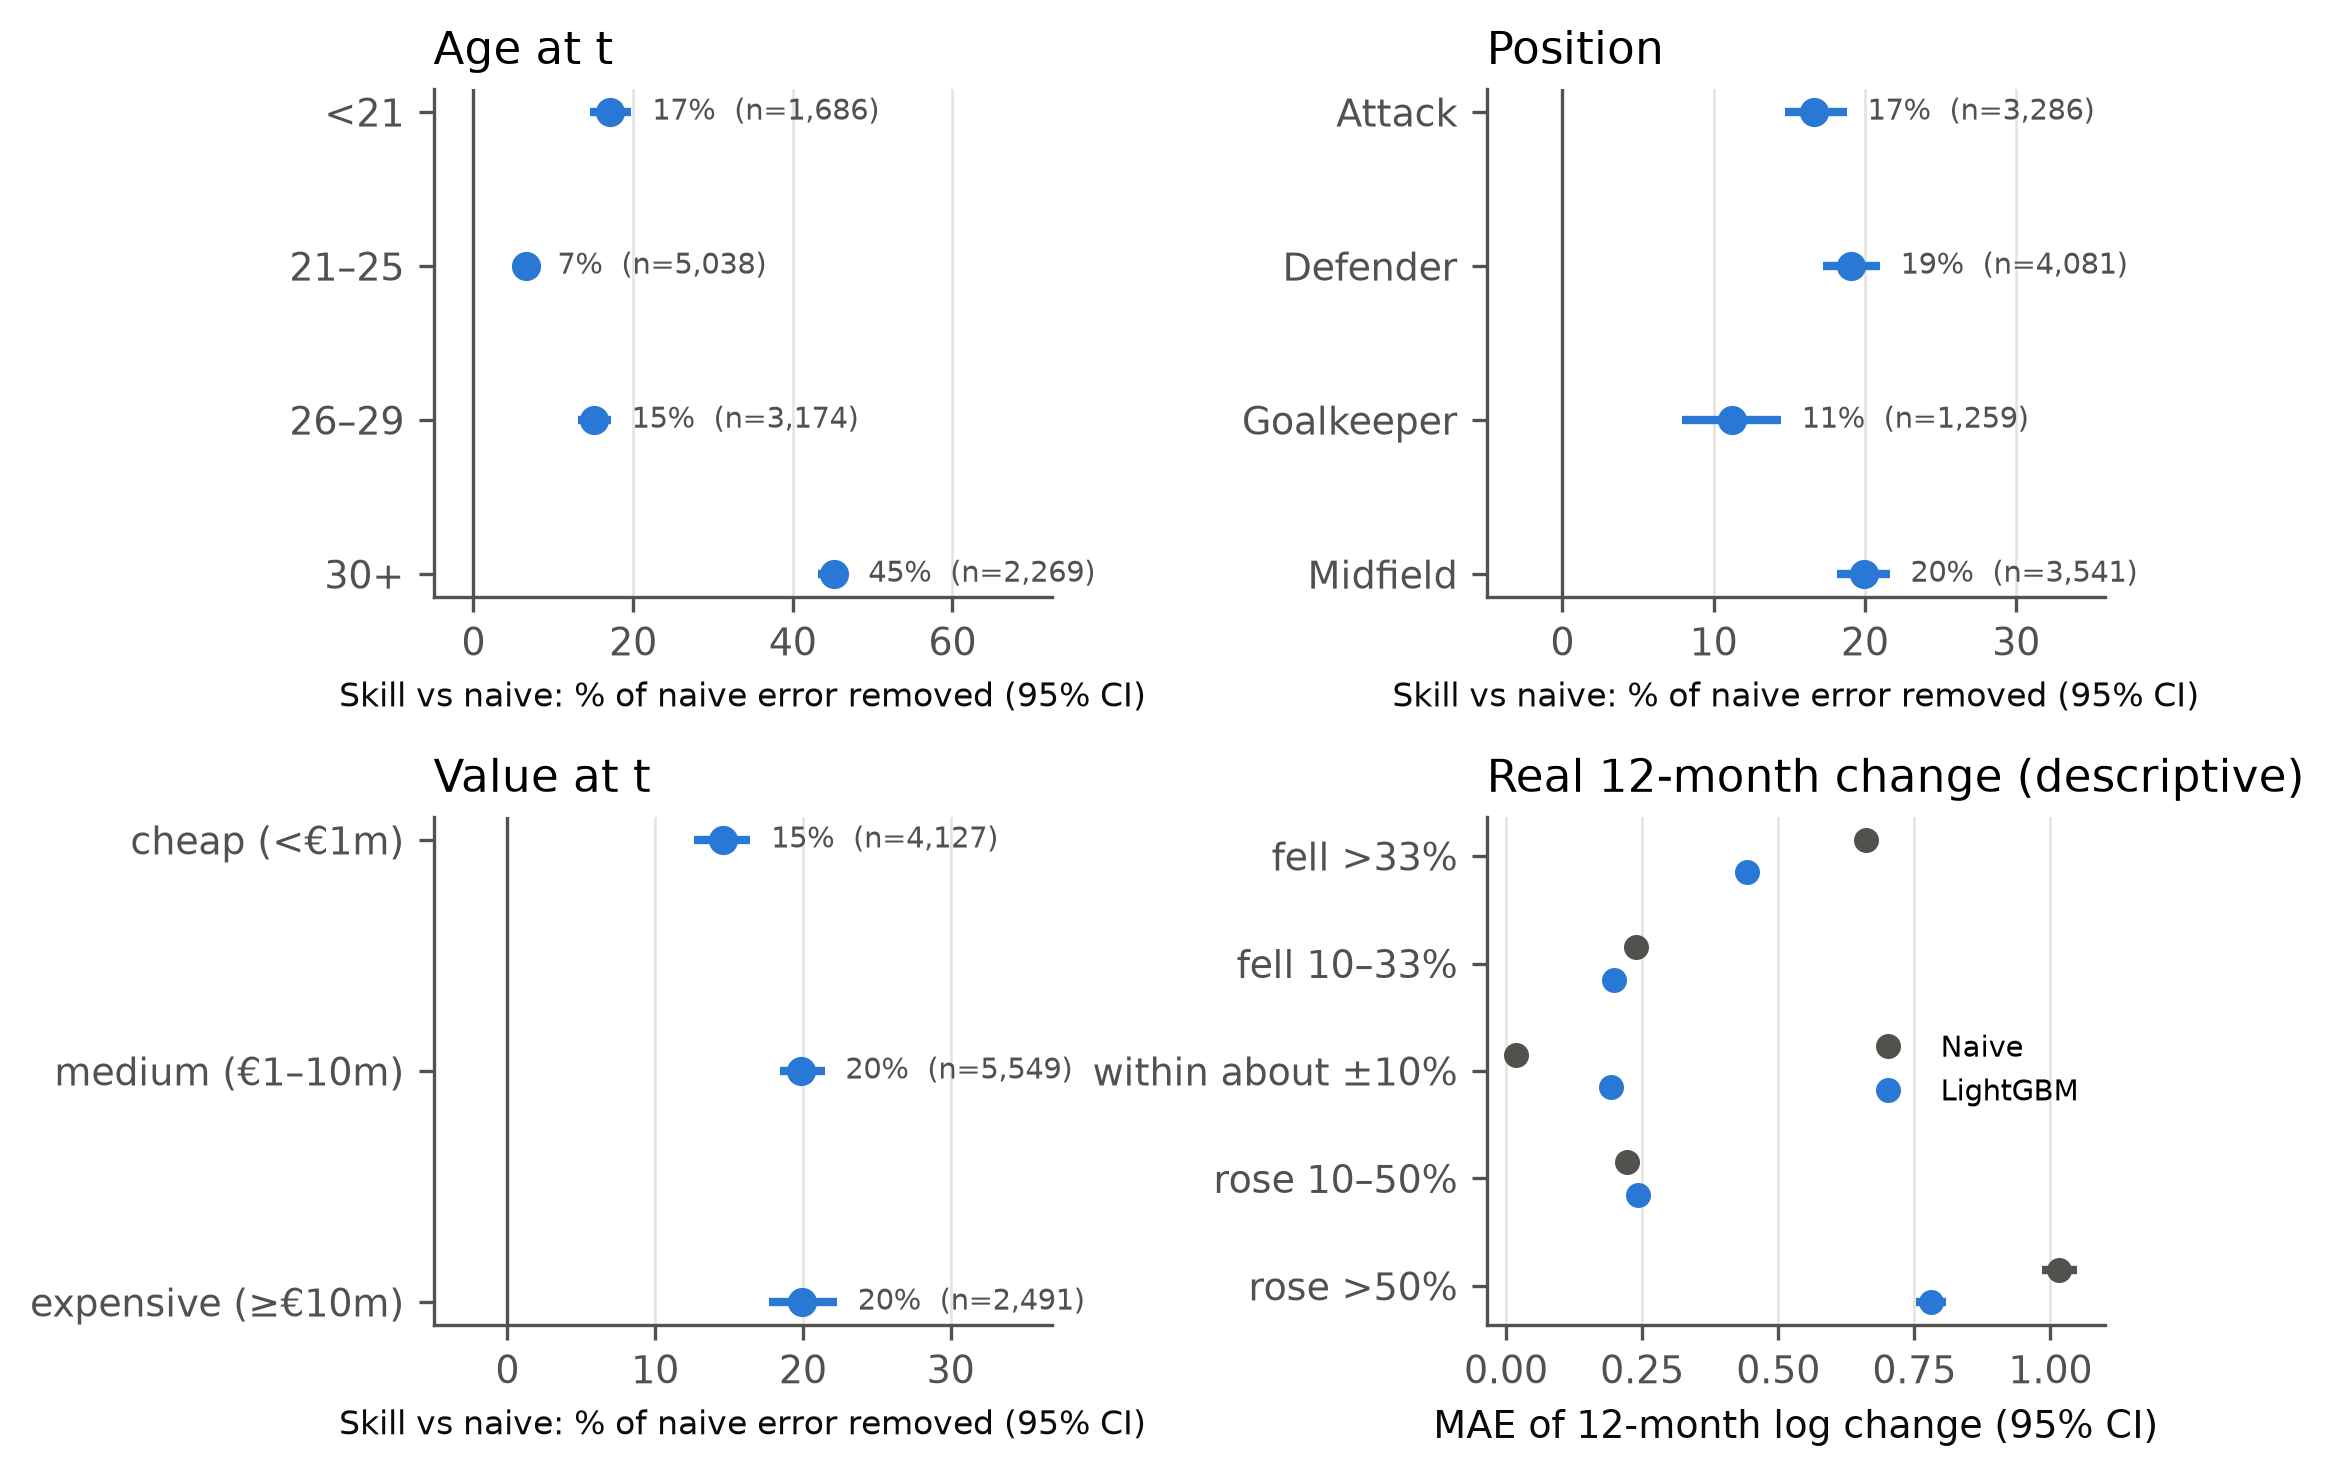
\includegraphics[width=0.72\textwidth]{fig07_gain_by_group.png}
\caption{LightGBM skill by group (test 2024/25, core leagues), measured against the no-change forecast (blue) and against the age $\times$ value curve (orange), with 95\% player-level bootstrap intervals. Bottom right: MAE of all three by size of the realised change (descriptive).}
\label{fig:groups}
\end{figure*}

\subsection{Where Does Machine Learning Help?}
Fig.~\ref{fig:groups} compares LightGBM with both references inside groups of players. Measured against no change, the gain looks largest for players aged 30 and over (\GrpVsNaiveC\%). Almost all of this is the routine decline that the curve already predicts. Against the curve, the gain for this group shrinks to \GrpVsCurveC\% \GrpVsCurveCCI.

Machine learning helps most for players under 21 (\GrpVsCurveU\% \GrpVsCurveUCI) and for falls in value, with \GrpVsCurveModFall\% for falls of 10 to 33\% and \GrpVsCurveBigFall\% for larger falls. On moderate rises of 10 to 50\% it is worse than the curve (\GrpVsCurveModRise\% \GrpVsCurveModRiseCI). Gains are similar across positions (\GrpPosVsCurveMin--\GrpPosVsCurveMax\%) and value levels.

Across the \NCoreLeagues{} core leagues, the gain over the curve is clearly positive in \CoreLgPosCount{} and negative in \CoreLgNeg. In the \NNewLeagues{} leagues never seen in training, LightGBM adds little beyond the curve, \NewVsCurve\% \NewVsCurveCI{} overall, and it is clearly positive in only \NewLgPosCount{} of them. Match data cover only \NewWindowCov\% of the 365-day performance window in these leagues. Even so, dropping the performance features makes the results worse (\NewNoPerfVsCurve\%).

\textit{Ranking.} The model also ranks players better than age does. Of its 10\% largest predicted rises, \RankRiseLGB\% actually rose, compared with \RankRiseYoung\% for the youngest 10\% of players (+\RankRiseDiff{} points, CI \RankRiseDiffCI). Of its 10\% largest predicted falls, \RankFallLGB\% actually fell, compared with \RankFallOld\% for the oldest 10\% (+\RankFallDiff{} points, CI \RankFallDiffCI).

\textit{Forecast intervals.} Before calibration, LightGBM quantile intervals cover \IntCovRaw\% \IntCovRawCI{} of true values instead of the target 80\%. Calibrating by age group brings coverage to \IntCovCal\% \IntCovCalCI. The intervals become \IntWidthIncrease\% wider, with a median width of \IntWidthCal\% of the value at $t$, and the mean pinball loss is \IntPinballCal, against \IntPinballRef{} for intervals built from the age $\times$ value percentiles. Under-21s are still slightly under-covered (\IntCovCalU\% \IntCovCalUCI). For players aged 30 and over, coverage is right at \IntCovCalC\%, but the misses lean one way. In \IntBelowC\% of cases the true value falls below the interval, and in only \IntAboveC\% above it.

\begin{figure}[t]
\centering
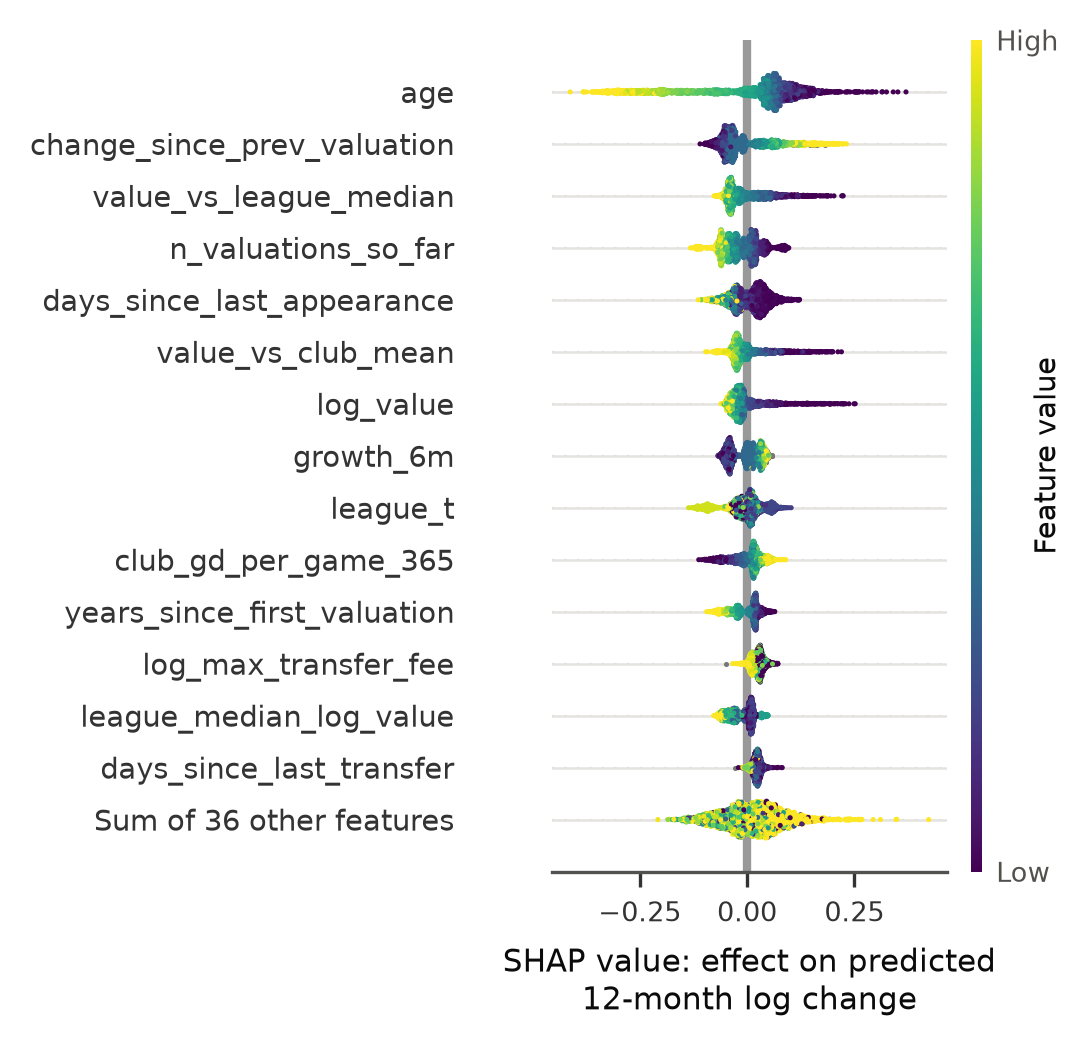
\includegraphics[width=0.92\columnwidth]{fig09_shap_beeswarm.png}
\caption{SHAP values of the 15 most important features (LightGBM, 3,000 test observations). Each dot is one observation; colour shows the feature value. Positive values push the forecast towards a rise.}
\label{fig:shap}
\end{figure}

\subsection{Explanations and Ablations}
We ran TreeSHAP~\cite{lundberg2017unified,lundberg2020trees} on 3,000 test observations (Fig.~\ref{fig:shap}). The top-ranked features are \ShapTopFive. Age pulls the forecast down steeply after about 28. Recent increases tend to continue. Players valued above their league or club median grow less, and long absences from matches point to a fall.

Table~\ref{tab:ablation} shows how much accuracy each group of features adds. Removing the value history hurts the most (+\AblHist), followed by performance (+\AblPerf) and player attributes (+\AblPlayer). Transfer features turned out to be of little use. Taking out the player's own transfer history, or the club's spending and income, changes the error by an amount we cannot tell apart from zero (club finance +\AblFin, n.s.), and in the SHAP ranking these features sit between \ShapFinRankMin{}rd and \ShapFinRankMax{}th out of \NFeatures. One reason is that club spending is strongly correlated with squad value (Spearman \SpendTotalValueCorr), which the model already uses. McHale and Holmes~\cite{mchale2023estimating} did find spending important, but their target was the fee itself. Position, sub-position, height and foot, the attributes taken from the 2026 snapshot, barely matter. Without them MAE$_\Delta$ goes up by \SnapDiff{} \SnapDiffCI.

\begin{table}[t]
\centering
\caption{Feature ablation (LightGBM, tuned settings, test 2024/25). $\Delta$MAE is the change versus the full model with a 95\% paired player-level bootstrap CI. ``n.s.'' means the CI contains 0. Snapshot attributes are position, sub-position, height and foot.}
\label{tab:ablation}
\footnotesize
\setlength{\tabcolsep}{3pt}
\resizebox{\columnwidth}{!}{\begin{tabular}{lrcll}
\toprule
Variant & Features & MAE$_\Delta$ & $\Delta$MAE [95\% CI] & Effect \\
\midrule
Full model & 50 & 0.3940 & -- & -- \\
\midrule
No value history & 39 & 0.4029 & 0.0089 [0.0070, 0.0109] & worse \\
No performance & 35 & 0.4004 & 0.0064 [0.0051, 0.0077] & worse \\
No player attributes & 44 & 0.3992 & 0.0052 [0.0039, 0.0066] & worse \\
No club/league & 36 & 0.3979 & 0.0039 [0.0021, 0.0056] & worse \\
No player transfer history & 46 & 0.3944 & 0.0004 [$-$0.0012, 0.0020] & n.s. \\
No club transfer finance (3) & 47 & 0.3946 & 0.0006 [$-$0.0001, 0.0012] & n.s. \\
Club spending removed & 49 & 0.3943 & 0.0003 [$-$0.0004, 0.0009] & n.s. \\
Snapshot attributes removed (4) & 46 & 0.3951 & 0.0011 [0.00003, 0.0021] & worse \\
Value history only & 11 & 0.4099 & 0.0158 [0.0130, 0.0187] & worse \\
Value history + age & 12 & 0.4045 & 0.0105 [0.0077, 0.0130] & worse \\
\bottomrule
\end{tabular}}
\end{table}


% =============================================================================
\section{Discussion}
Because the target is a Transfermarkt estimate, a model partly learns the habits of the people who set those estimates. Two of our results point to a lot of the predictable movement being routine. Older players get marked down and young ones get marked up, year after year. That is why a plain age $\times$ value curve is so hard to beat, and why the big gain for players over 30 vanishes once the baseline knows their age. What machine learning adds on top is smaller but steady, and it shows up mainly for young players and for players about to lose value.

To check whether this carries over to real money, we matched the forecasts against actual fees for the \FeeN{} test observations where the player was sold within 12 months (\FeePlayers{} players). The Spearman correlation between the predicted change and $\log(\text{fee}/\text{value at }t)$ is \FeeRhoLGB{} \FeeRhoLGBCI{} for LightGBM and \FeeRhoCurve{} \FeeRhoCurveCI{} for the curve, a clear difference of \FeeRhoDiffCurve{} \FeeRhoDiffCurveCI. Age alone, however, reaches \FeeRhoAge{} \FeeRhoAgeCI, and LightGBM is not clearly better than that (difference \FeeRhoDiffAge{} \FeeRhoDiffAgeCI). Even the true change in the Transfermarkt value correlates only \FeeRhoTrue{} with fees. Forecasting the community value is useful, then, but it tells only part of the story about real prices.

\subsection{Limitations}\label{sec:limits}
We forecast a community estimate, which is only partly linked to transfer fees~\cite{coates2022wisdom}. Among core-league test observations with a fully observable window, \DropRateTest\% have no valuation 10 to 14 months later. These dropped cases are not mostly falls. Within 18 months, \DropFell\% of them fell and \DropRose\% rose, compared with \KeptFell\% and \KeptRose\% for the observations we kept. Dropped players under 21, however, rose much less (median log change \DropYoungMedian{} vs.\ \KeptYoungMedian), so forecasts for young players who leave coverage may be too optimistic.

Match data for the full period exist for only \NCoreLeagues{} European leagues. In the other \NNewLeagues{} leagues, \NewZeroMin\% of test observations show zero minutes, against \CoreZeroMin\% in the core leagues. Contract, wage and injury data are missing altogether. Position, height and foot are taken from the 2026 snapshot, but removing them hardly changes accuracy. Even after calibration, intervals for under-21s are a bit too narrow, and for older players most misses are on the low side. Our GRU is small and sees only valuation histories, so it says little about what a stronger sequence model could do.

\section{Conclusion}
Can public Transfermarkt data be used to benchmark value forecasts? Yes, but two repairs come first. The 2026 snapshot columns have to go, and each player's club history has to be rebuilt from transfers and appearances. The split must also follow time. Once that is done, age and current value explain most of what can be predicted a year out. Boosted trees still improved on them in each of the six seasons, mostly for under-21s and for players heading for a drop, but much less in leagues they were not trained on. We would next like to add contract and injury records, which the Kaggle data do not have, and to check the forecasts against real fees instead of the community estimate alone.

\section*{Data and Code Availability}
All data come from the public Kaggle dataset~\cite{kaggle_transfermarkt}, and the exact version can be checked with its SHA-256 checksums. One script verifies the version and regenerates the \NResultTables{} result tables and \NFigures{} figures. \ifanonymous
To keep the review anonymous we do not give the code link here. It will be released once the review is over.
\else
The code is available at \url{https://github.com/t-raisa/football-market-value}.
\fi

% Balance the two columns on the last page (submission version). The camera-ready version is balanced without a break.
\ifanonymous\IEEEtriggeratref{13}\fi
\bibliographystyle{IEEEtran}
\bibliography{references}

\end{document}
